% ======================================================================
%  Chapter 6 — Dirac Cones of Light
% ======================================================================

\section{Why Dirac points matter}
\label{sec:ch6-why-dirac}

In the previous chapter we learned that a nonzero \emph{Chern number}
requires time-reversal symmetry to be broken.  With time reversal
preserved, the Berry curvature satisfies $\Omega_n(\kvec)=-\Omega_n(-\kvec)$
and can be locally nonzero---for example near valleys where inversion
symmetry is broken---but its integral over the full Brillouin zone
vanishes
\cite{noh2017observation}.  Concentrated sources of Berry flux somewhere in the Brillouin
zone are therefore needed for any topological band.
Where does this Berry flux come from?

The answer, in essentially all known photonic topological systems, is
\emph{Dirac points}: isolated degeneracies in the band structure where
two bands touch with a linear (conical) dispersion.  These degeneracies
are the ``monopoles'' of Berry curvature in momentum space.  When a
perturbation gaps a Dirac point, the Berry flux that was compressed
into the degeneracy spreads into a concentrated peak of Berry curvature,
and the two split bands acquire equal and opposite contributions to
their Chern numbers.

In this chapter we explain how Dirac points arise in two-dimensional
photonic crystals from symmetry, derive their local dispersion from a
two-mode reduction of the Maxwell eigenproblem, and prepare the ground
for the topological gap opening of \chref{ch:breaking-tr}.  The treatment
follows the original analysis of Haldane and Raghu \cite{haldane2008possible,khanikaev2013photonic}
and the comprehensive review by Ozawa et~al.\ \cite{ozawa2018topological},
adapted to the Maxwell-first framework of this book.

\section{Symmetry protection of Dirac degeneracies}
\label{sec:ch6-symmetry}

\subsection{The real-symmetric condition}
\label{sec:ch6-real-symmetric}

Recall from \chref{ch:geometry-bands} that when both time-reversal
($\Top$) and spatial inversion ($\Pop$) symmetries are present, the
Berry curvature vanishes identically:
\begin{equation}\label{eq:ch6-zero-curvature}
  \Top + \Pop \quad\Longrightarrow\quad
  \Omega_n(\kvec) = 0\;\;\text{for all } \kvec\,.
\end{equation}
This means that we can choose a \emph{real} gauge: the cell-periodic
eigenmodes $\mathbf{u}_{n\kvec}(\rvec)$ can be made real-valued for all
$\kvec$.  The Maxwell eigenvalue problem then becomes a
\emph{real-symmetric} generalised eigenproblem rather than a
complex-Hermitian one.

This distinction is crucial for degeneracies.  In a complex-Hermitian
eigenproblem, an ``accidental'' degeneracy between two bands requires
the simultaneous vanishing of \emph{three} real parameters (the real
part, imaginary part, and diagonal difference of the off-diagonal matrix
element).  In two dimensions, we have only two parameters $(k_x,k_y)$,
so a generic complex-Hermitian system has no band degeneracies in 2D.

In a \emph{real-symmetric} eigenproblem, a degeneracy requires the
vanishing of only \emph{two} real parameters (the off-diagonal element
and the diagonal difference).  Two conditions in two unknowns
$(k_x,k_y)$ generically have isolated point solutions.  These isolated
degeneracies are the Dirac points.

To make this concrete, consider a generic $2\times 2$ real-symmetric
matrix
\begin{equation}\label{eq:ch6-vNW-matrix}
  \mathbf{H}(k_x,k_y)
  = \begin{pmatrix}
    a(k_x,k_y) & b(k_x,k_y) \\
    b(k_x,k_y) & c(k_x,k_y)
  \end{pmatrix}.
\end{equation}
Its eigenvalues are
$\lambda_\pm = \frac{1}{2}(a+c)\pm\frac{1}{2}\sqrt{(a-c)^2+4b^2}$,
which become degenerate when $a=c$ and $b=0$ simultaneously.  These two
equations in two unknowns $(k_x,k_y)$ generically have isolated
solutions---the Dirac points.  If the matrix were complex Hermitian,
the off-diagonal element would be $b_R+\ii b_I$, requiring three
conditions ($a=c$, $b_R=0$, $b_I=0$) in two unknowns, which generically
have no solution.

\begin{remark}
This argument, due to von~Neumann and Wigner in the electronic context
\cite{ozawa2018topological},
explains why Dirac points are \emph{generic} (symmetry-allowed, not
fine-tuned) in 2D photonic crystals with both $\Top$ and $\Pop$
symmetry.  Breaking either symmetry removes the reality condition and
generically gaps the degeneracy.
\end{remark}

\subsection{Hexagonal lattice and the K, K-prime points}
\label{sec:ch6-hexagonal}

The hexagonal (triangular) lattice, with point group $C_{6v}$, is the
natural host for photonic Dirac points.  The first Brillouin zone is a
regular hexagon, whose six corners fall into two inequivalent sets:
three $K$ points and three $K'$ points, related by time reversal
($K'=-K$ modulo reciprocal lattice vectors).

At each $K$ point, the little group (the subgroup of $C_{6v}$ that
leaves $\kvec_K$ invariant) is $C_{3v}$, which has two-dimensional
irreducible representations.  Modes transforming under such a
representation are doubly degenerate at $K$.  When these degenerate
modes belong to adjacent bands, they form a Dirac point.

\begin{remark}
  The square lattice ($C_{4v}$) can also host Dirac points at the $M$
  point under appropriate conditions, but the hexagonal lattice provides
  the cleanest and most widely studied example.  The connection to
  graphene---a hexagonal lattice of carbon atoms whose electronic
  structure has Dirac cones at $K$ and $K'$---was the direct inspiration
  for Haldane and Raghu's photonic construction \cite{haldane2008possible,plotnik2011experimental}.
\end{remark}

\section{Nearly-free-photon analysis}
\label{sec:ch6-nfp}

Following Haldane and Raghu, we construct a photonic Dirac point
analytically using a ``nearly-free-photon'' approximation---the photonic
analog of the nearly-free-electron model in solid-state physics.

\subsection{Setup}
\label{sec:ch6-nfp-setup}

Consider a 2D photonic crystal with uniform isotropic permeability
$\mu(\rvec)=\mu_0$ and a spatially modulated permittivity
\begin{equation}\label{eq:ch6-eps-modulated}
  \varepsilon(\rvec) = \bar\varepsilon\bigl(1+\lambda\,V_G(\rvec)\bigr)\,,
\end{equation}
where $\lambda\ll 1$ is the modulation strength and
\begin{equation}\label{eq:ch6-VG}
  V_G(\rvec) = \frac{2}{3}\sum_{n=1}^{3}\cos(\Gvec_n\cdot\rvec)
\end{equation}
is a potential with the periodicity of a hexagonal lattice.  Here
$\Gvec_1$, $\Gvec_2$, $\Gvec_3$ are three reciprocal lattice vectors
of equal length $|\Gvec|=4\pi/(\sqrt{3}\,a)$, rotated by $120^\circ$
relative to each other.

We work at $k_z=0$, so the TE and TM polarisations decouple
(\secref{sec:ch4-te-tm}).  We specialise to the TE set
$\{E_x,E_y,H_z\}$.

\subsection{Free-photon dispersion at the Brillouin-zone corner}
\label{sec:ch6-free-photon}

The six corners of the hexagonal Brillouin zone are at
$\pm\kvec_{K_n}$, where
$\kvec_{K_1}=(\Gvec_2-\Gvec_3)/3$, etc., with
$|\kvec_K|=|\Gvec|/\sqrt{3}$.  Since $\kvec_{K_2}-\kvec_{K_1}=\Gvec_3$,
the three wavevectors $\kvec_{K_1}$, $\kvec_{K_2}$, $\kvec_{K_3}$ are
equivalent as Bloch vectors.

At $\lambda=0$ (uniform medium), the TE mode at wavevector $\kvec$ has
the free-photon dispersion $\omega=c_0|\kvec|$, where
$c_0=c/\sqrt{\bar\varepsilon}$.  At the Brillouin-zone corner
$\kvec=\kvec_K$, three free-photon plane waves (corresponding to
$\kvec_K$, $\kvec_K+\Gvec_1$, $\kvec_K+\Gvec_2$, which all have the
same $|\kvec+\Gvec|=|\kvec_K|$) are degenerate at frequency
$\omega_0=c_0|\kvec_K|$.

\subsection{Splitting by the periodic potential}
\label{sec:ch6-splitting}

Turning on the periodic modulation $\lambda\neq 0$ lifts the
threefold degeneracy.  In degenerate perturbation theory, we must
diagonalise the $3\times 3$ matrix of the perturbation
$\delta\Maxop=-(\omega_D\lambda\bar\varepsilon/2)V_G(\rvec)$ within the
three-mode subspace at $\kvec=\kvec_K$.  Denoting the three degenerate
free-photon states as $|\alpha\rangle$, $\alpha=1,2,3$, the coupling
matrix has elements \cite{haldane2008possible}
\begin{equation}\label{eq:ch6-coupling-matrix}
  D_{\alpha\beta}
  = \frac{\omega_D\lambda}{2}
  \int_{\Omega}V_G(\rvec)\,
  \mathbf{u}^*_\alpha(\rvec)\cdot
  \bar\varepsilon\,\mathbf{u}_\beta(\rvec)\,\dd^2 r\,,
\end{equation}
where the integral runs over one unit cell~$\Omega$.  The hexagonal
symmetry $C_{3v}$ acting on the three plane-wave modes permutes them
cyclically, so $D_{\alpha\beta}$ inherits the structure
\begin{equation}\label{eq:ch6-3x3-matrix}
  \mathbf{D} = \frac{\omega_D\lambda}{4}
  \begin{pmatrix}
    0 & 1 & 1 \\ 1 & 0 & 1 \\ 1 & 1 & 0
  \end{pmatrix}.
\end{equation}
The eigenvalues of \eqref{eq:ch6-3x3-matrix} are
$-\omega_D\lambda/4$ (doubly degenerate) and
$+\omega_D\lambda/2$ (non-degenerate).  The threefold degeneracy
therefore splits into a \emph{Dirac doublet}, whose frequency is
shifted down to
\begin{equation}\label{eq:ch6-omega-D}
  \omega_D
  = c_0|\kvec_K|\bigl(1-\tfrac{\lambda}{4}+O(\lambda^2)\bigr)\,,
\end{equation}
and a \emph{singlet}, shifted up to
\begin{equation}\label{eq:ch6-omega-singlet}
  \omega_s
  = c_0|\kvec_K|\bigl(1+\tfrac{\lambda}{2}+O(\lambda^2)\bigr)\,,
\end{equation}
separated from the doublet by a gap of order $\lambda$.

At momenta $\kvec=\kvec_K+\delta\kvec$ away from the zone corner,
first-order $\kvec\cdot\mathbf{p}$ perturbation theory within the
two-mode doublet gives the conical dispersion
\begin{equation}\label{eq:ch6-dirac-dispersion}
  \omega_\pm(\kvec) = \omega_D \pm v_D|\delta\kvec| + O(|\delta\kvec|^2)\,,
\end{equation}
with the Dirac velocity $v_D=c_0/2+O(\lambda)$.  This linear
dispersion is the hallmark of a Dirac cone: it is locally identical to
the spectrum of a massless two-dimensional relativistic particle.

\subsection{Symmetry constraints on the coupling matrix}
\label{sec:ch6-symmetry-coupling}

The simple structure of \eqref{eq:ch6-3x3-matrix} is not accidental.
The three reciprocal lattice vectors $\Gvec_1,\Gvec_2,\Gvec_3$
transform into one another under the threefold rotation $C_3$ of the
hexagonal lattice, and $V_G$ respects this symmetry.  Therefore the
overlap integral $D_{\alpha\beta}$ depends only on whether $\alpha$
and $\beta$ are equal or unequal: $D_{\alpha\alpha}=d_0$ and
$D_{\alpha\neq\beta}=d_1$.  The trace and off-diagonal parts can be
removed by a constant shift, leaving the traceless matrix
\eqref{eq:ch6-3x3-matrix} whose double eigenvalue is protected by the
two-dimensional irreducible representation $E$ of $C_{3v}$.

Time-reversal symmetry enters via the reality constraint:
because $\Top$ maps $\kvec_K$ to $\kvec_{K'}=-\kvec_K$ and simultaneously
complex-conjugates the eigenmode, the coupling matrix at $K$ is
real-symmetric (consistent with \eqref{eq:ch6-3x3-matrix}).  This
reality condition is what makes the degeneracy \emph{robust}: perturbing
the matrix within the space of real-symmetric matrices cannot split a
twofold eigenvalue because real-symmetric $2\times 2$ degeneracies have
codimension~2 in two-parameter space, exactly matching the
dimensionality of the Brillouin zone.

By contrast, if one breaks the $C_3$ symmetry while preserving the
reality condition, the off-diagonal elements $d_1$ between different
pairs of modes become unequal, generically splitting all three
eigenvalues and removing the degeneracy entirely.  The Dirac point is
therefore protected specifically by the combination of $C_3$ rotation
and time reversal, not by any single symmetry alone
\cite{ozawa2018topological}.

\section{The two-mode Maxwell reduction}
\label{sec:ch6-two-mode}

Near the Dirac point, the physics is captured by a $2\times 2$
effective equation obtained by projecting the full Maxwell eigenproblem
onto the two degenerate modes.

\subsection{Projection onto the degenerate subspace}
\label{sec:ch6-projection}

Let $|\mathbf{u}_+(\kvec_K)\rangle$ and $|\mathbf{u}_-(\kvec_K)\rangle$ be
the two degenerate cell-periodic eigenmodes at the Dirac point,
normalised so that
$\langle\mathbf{u}_\sigma|\Mgmat(\omega_D)|\mathbf{u}_{\sigma'}\rangle
=B_0\,\delta_{\sigma\sigma'}$.

For $\kvec=\kvec_K+\delta\kvec$ with $|\delta\kvec|\ll|\kvec_K|$,
first-order $\kvec\cdot\mathbf{p}$ perturbation theory gives the
$2\times 2$ effective eigenvalue equation
\begin{equation}\label{eq:ch6-effective-dirac}
  \boxed{%
  v_D\bigl(\delta k_x\,\sigma_x + \delta k_y\,\sigma_y\bigr)
  |\psi\rangle
  = \delta\omega\,|\psi\rangle\,,}
\end{equation}
where $\delta\omega=\omega-\omega_D$, $\sigma_x$ and $\sigma_y$ are
Pauli matrices acting on the two-mode subspace, and $v_D>0$ is the
Dirac velocity determined by the matrix elements of the velocity
operator between the two degenerate modes:
\begin{equation}\label{eq:ch6-vD}
  v_D = \frac{1}{B_0}
  \bigl|\langle\mathbf{u}_+|\partial_{k_x}\Maxop|\mathbf{u}_-\rangle
  \bigr|\,.
\end{equation}

\subsection{Dirac dispersion and eigenstates}
\label{sec:ch6-dirac-eigenstates}

The eigenvalues of \eqref{eq:ch6-effective-dirac} are
\begin{equation}\label{eq:ch6-dirac-eval}
  \delta\omega_\pm = \pm v_D|\delta\kvec|\,,
\end{equation}
reproducing the conical dispersion \eqref{eq:ch6-dirac-dispersion}.
The eigenstates are
\begin{equation}\label{eq:ch6-dirac-evec}
  |\psi_\pm(\delta\kvec)\rangle
  = \frac{1}{\sqrt{2}}
  \begin{pmatrix} 1 \\ \pm\ee^{\ii\phi_\kvec} \end{pmatrix},
  \qquad \phi_\kvec = \arg(\delta k_x + \ii\,\delta k_y)\,.
\end{equation}
As $\delta\kvec$ traces a circle around the Dirac point, the angle
$\phi_\kvec$ winds by $2\pi$ and the eigenstate acquires a Berry phase
of $\pm\pi$.

\subsection{Berry curvature at a Dirac point}
\label{sec:ch6-dirac-berry}

The Berry curvature of the gapless Dirac cone is concentrated at the
degeneracy point.  Using the Kubo formula
(\eqnref{eq:ch5-kubo-formula}), the Berry curvature of the upper band
diverges as $|\delta\kvec|\to 0$:
\begin{equation}
  \Omega_+(\delta\kvec)
  \sim \frac{1}{2|\delta\kvec|^2}
  \quad\text{as } |\delta\kvec|\to 0\,.
\end{equation}
The total Berry flux through a small disc around the Dirac point is
$\pm\pi$, which is the Berry phase acquired by the eigenstate on
a loop encircling the degeneracy.  However, this is a \emph{gapless}
system and the Chern number is not defined until the degeneracy is
lifted---which is the subject of the next chapter.

\section{Dirac points in realistic photonic crystals}
\label{sec:ch6-realistic}

The nearly-free-photon analysis gives the essential physics but requires
$\lambda\ll 1$, where the Dirac-point frequency $\omega_D$ lies close
to other bands and is not well isolated.  In realistic photonic crystals
with large dielectric contrast, the Dirac points can be frequency-isolated
within a substantial gap of the opposite polarisation, making them
suitable hosts for topological gap opening.

Haldane and Raghu noted that a hexagonal array of high-permittivity
rods ($\varepsilon_r=14$, filling fraction $f=0.431$) in air produces a
band structure where the second and third TE bands touch at Dirac points
at the Brillouin-zone corners $K$ and $K'$, and the Dirac frequency
$\omega_D$ lies within a large gap of the TM spectrum
\cite{haldane2008possible}.  This frequency isolation is crucial: it
ensures that the Dirac-point modes are not degenerate with any other
$k_z=0$ modes, so that the topological gap opening can proceed without
interference from other bands.

\section{Pairs of Dirac points and the fermion-doubling theorem}
\label{sec:ch6-pairs}

A fundamental property of Dirac points in a 2D Brillouin zone is that
they always come in \emph{pairs}: one at $K$ and one at $K'=-K$.  This
is the photonic version of the Nielsen--Ninomiya (fermion-doubling)
theorem, which states that the total chirality of all Dirac points in a
compact Brillouin zone must vanish.

To see how Dirac-point pairing controls the Chern number, introduce
a valley index $\tau=\pm 1$ labelling $K$ ($\tau=+1$) and
$K'$ ($\tau=-1$).  Near valley $\tau$ the effective Hamiltonian is
\begin{equation}\label{eq:ch6-valley-hamiltonian}
  H_\tau(\delta\kvec)
  = v_D\bigl(\tau\,\delta k_x\,\sigma_x
  + \delta k_y\,\sigma_y\bigr)
  + \Delta_\tau\,\sigma_z\,,
\end{equation}
where $\Delta_\tau$ is the mass induced by a perturbation that opens a
gap.  The chirality factor $\tau$ multiplies $\delta k_x$: physically,
$K$ and $K'$ carry \emph{opposite} winding numbers.  Both gapless cones
have a Berry phase of $\pi$, but the opposite chiralities cause the two
valleys to contribute to the Chern number with a relative sign.
Explicitly, from the massive Dirac Berry curvature
(derived in \secref{sec:ch7-berry-curvature}):
\begin{equation}\label{eq:ch6-valley-chern-contribution}
  C_-^{K}=-\frac{\operatorname{sgn}(\Delta_K)}{2}\,,
  \qquad
  C_-^{K'}=+\frac{\operatorname{sgn}(\Delta_{K'})}{2}\,,
\end{equation}
so the total lower-band Chern number is
\begin{equation}\label{eq:ch6-total-chern-valleys}
  \Chern_-
  = \frac{\operatorname{sgn}(\Delta_{K'})
         -\operatorname{sgn}(\Delta_K)}{2}\,.
\end{equation}
Two physically distinct gap-opening mechanisms now follow.

\emph{Time-reversal breaking} (Haldane/gyrotropic mass).---The
perturbation gives \emph{opposite}-sign masses at the two valleys,
$\Delta_K=-\Delta_{K'}$, because the gyrotropic coupling picks up the
chirality factor $\tau$.  The valley contributions reinforce:
$\Chern_-=\pm 1$, and the system supports a chiral edge mode
(\chref{ch:breaking-tr}).

\emph{Inversion breaking} (Semenoff mass).---The perturbation gives
\emph{same}-sign masses, $\Delta_K=\Delta_{K'}$, and $\Chern_-=0$.
However, the half-integer valley contributions $C_-^{K}$ and $C_-^{K'}$
are individually nonzero, defining a \emph{valley Chern number}
(\chref{ch:valleys}).

This valley-indexed structure is the central organising principle for
all of Parts~II and~III.


\begin{figure}[t]
  \centering
  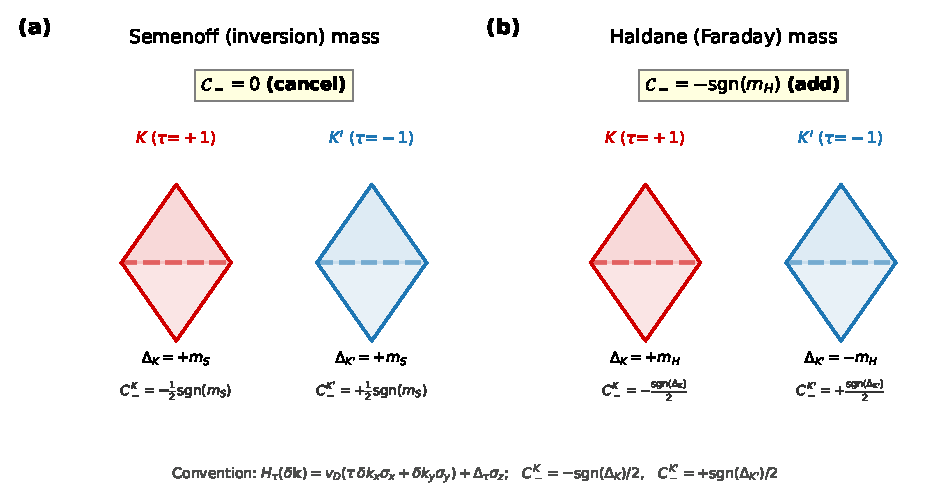
\includegraphics[width=0.92\textwidth]{figures/fig_ch06_valley_mass_taxonomy_step236.pdf}
  \caption{Valley Chern-number bookkeeping for the two gap-opening
  mechanisms.  \textbf{(a)}~Semenoff (inversion) mass: both valleys
  receive the same mass $\Delta_K=\Delta_{K'}=m_S$, so the valley
  contributions $C_-^K=-\operatorname{sgn}(m_S)/2$ and
  $C_-^{K'}=+\operatorname{sgn}(m_S)/2$ cancel, giving $\Chern_-=0$.
  \textbf{(b)}~Haldane (Faraday) mass: the gyrotropic coupling
  assigns opposite-sign masses $\Delta_K=+m_H$, $\Delta_{K'}=-m_H$,
  so the valley contributions reinforce to give
  $\Chern_-=-\operatorname{sgn}(m_H)$.  The convention follows
  \eqref{eq:ch6-effective-dirac} with $\tau_K=+1$, $\tau_{K'}=-1$.}
  \label{fig:ch06-valley-mass-taxonomy}
\end{figure}
\section{Derivation of the Dirac velocity}
\label{sec:ch6-vD-derivation}

The Dirac velocity $v_D$ appearing in \eqref{eq:ch6-effective-dirac}
is not a phenomenological parameter.  It is determined entirely by
the Maxwell eigenmodes at the $K$ point through the electromagnetic
energy inner product.  Deriving its explicit form from $\kvec\cdot\mathbf{p}$
perturbation theory within the Maxwell framework illustrates the
power of the approach developed in Chapters~2--5.

\subsection{The electromagnetic velocity operator}
\label{sec:ch6-velocity-operator}

Starting from the Bloch-periodic Maxwell eigenproblem
$\Maxop(\kvec)\mathbf{u}_{n\kvec}=\omega_{n\kvec}\Mgmat\mathbf{u}_{n\kvec}$,
differentiate both sides with respect to $k_a$ ($a=x,y$).
Projecting onto a different eigenmode $\mathbf{u}_{m\kvec}$ with
$m\neq n$ and using the orthogonality
$\emip{\mathbf{u}_m}{\mathbf{u}_n}=\delta_{mn}$ gives the
electromagnetic Hellmann--Feynman relation
\begin{equation}\label{eq:ch6-HF-offdiag}
  \frac{1}{B_0}\emip{\mathbf{u}_m}{\partial_{k_a}\Maxop\;\mathbf{u}_n}
  = (\omega_n-\omega_m)\,
  \emip{\mathbf{u}_m}{\Mgmat\,\partial_{k_a}\mathbf{u}_n}\,,
\end{equation}
where $B_0$ is the energy normalisation and $\partial_{k_a}\Maxop$
acts on the cell-periodic part of the Bloch wave.  The left-hand side
defines the matrix element of the velocity operator
$\hat{v}_a\equiv\Mgmat^{-1}\partial_{k_a}\Maxop$, weighted by the
energy metric \cite{gangaraj2016berry}.  This operator plays exactly
the role of the momentum operator $\hat{p}/m$ in the electronic
$\kvec\cdot\mathbf{p}$ theory.

\subsection{Degenerate perturbation at the K point}
\label{sec:ch6-degenerate-kp}

At $\kvec=\kvec_K$ the two modes $\mathbf{u}_\pm$ are degenerate at
$\omega_D$, so the denominator in \eqref{eq:ch6-HF-offdiag} vanishes
and the non-degenerate formula cannot be used.  Instead, expand
the operator to first order in $\delta\kvec$:
\begin{equation}\label{eq:ch6-Maxop-expand}
  \Maxop(\kvec_K+\delta\kvec)
  = \Maxop(\kvec_K)
  + \delta k_x\,\partial_{k_x}\Maxop\big|_K
  + \delta k_y\,\partial_{k_y}\Maxop\big|_K
  + O(|\delta\kvec|^2)\,.
\end{equation}
Within the two-mode subspace, the first-order perturbation matrix is
\begin{equation}\label{eq:ch6-V-matrix}
  \mathcal{V}_{\sigma\sigma'}(\delta\kvec)
  = \frac{1}{B_0}
  \sum_{a=x,y}\delta k_a\,
  \emip{\mathbf{u}_\sigma}{\partial_{k_a}\Maxop\;\mathbf{u}_{\sigma'}}\,.
\end{equation}
The threefold rotation $C_3$ at the $K$ point cyclically permutes
the basis modes and constrains the matrix elements.
In particular, $C_3$ forces the diagonal elements to vanish at
first order in $\delta\kvec$ (they contribute to the quadratic
correction).  The off-diagonal element is fixed by the requirement
that $\mathcal{V}$ transforms as the two-dimensional $E$
representation of $C_{3v}$, giving
\begin{equation}\label{eq:ch6-V-offdiag}
  \mathcal{V}_{+-} = v_D(\delta k_x - \ii\,\delta k_y)\,,
  \qquad
  \mathcal{V}_{-+} = v_D(\delta k_x + \ii\,\delta k_y)\,,
\end{equation}
where the Dirac velocity is the real, positive quantity
\begin{equation}\label{eq:ch6-vD-formula}
  \boxed{%
  v_D = \frac{1}{B_0}
  \bigl|\emip{\mathbf{u}_+}{\partial_{k_x}\Maxop\;\mathbf{u}_-}\bigr|\,.}
\end{equation}
Substituting into $\mathcal{V}=\delta\omega\,\mathbf{I}$ recovers
the massless Dirac equation \eqref{eq:ch6-effective-dirac}
\cite{haldane2008reflection}.

\subsection{Numerical estimates}
\label{sec:ch6-numerical-vD}

For a hexagonal lattice of high-permittivity dielectric rods
($\varepsilon_r=12$, filling fraction $f=0.3$) in air, a plane-wave
expansion with 169 plane waves gives the Dirac frequency
$\omega_D a/(2\pi c)\approx 0.36$ and a Dirac velocity
$v_D\approx 0.45\,c/\sqrt{\bar\varepsilon}$
\cite{haldane2008possible,ozawa2018topological}.  The deviation from
the nearly-free-photon prediction $v_D=c_0/2$ reflects the finite
dielectric contrast, which distorts the mode profiles from pure
plane waves and modifies the overlap integral in
\eqref{eq:ch6-vD-formula}.

Reducing the rod permittivity toward $\varepsilon_r\to 1$
makes the modes more plane-wave-like and pushes $v_D$ toward
$c_0/2$, confirming the nearly-free-photon limit.  Conversely,
increasing the contrast beyond $\varepsilon_r\approx 15$ brings the
Dirac frequency close to higher bands and eventually destroys the
isolated Dirac cone, as the two-mode approximation breaks down.

\subsection{Physical meaning of the Dirac velocity}
\label{sec:ch6-vD-physical}

The Dirac velocity $v_D$ sets three experimentally accessible
quantities.  First, the group velocity of wavepackets near the Dirac
frequency: $|\mathbf{v}_g|=v_D$ for all propagation directions,
a consequence of the isotropic conical dispersion enforced by $C_3$.
Second, the density of states near $\omega_D$ scales as
$\rho(\omega)\propto|\omega-\omega_D|/v_D^2$, vanishing linearly at
the Dirac frequency---the photonic analog of the vanishing density of
states in graphene.  Third, when the Dirac cone is gapped by a mass
$\kappa$ (Chapter~\ref{ch:breaking-tr}), the edge-mode group velocity
inside the topological gap is approximately $v_D$, so the Dirac
velocity directly determines the bandwidth and propagation speed of
the one-way edge channel \cite{ozawa2018topological}.

\section{From Dirac cones to topological gaps: a summary}
\label{sec:ch6-summary}

This chapter has established three results that form the foundation for
Part~II of the book.

The first result is that Dirac points are generic features of 2D
photonic crystals with $C_3$ (or $C_6$) rotational symmetry and
time-reversal invariance.  The real-symmetric structure of the Maxwell
eigenproblem under these symmetries reduces the codimension of band
degeneracies from three (complex Hermitian) to two (real symmetric),
matching the two-dimensional Brillouin zone and yielding isolated
point degeneracies.

The second result is that the local physics near a Dirac point is
captured by a $2\times 2$ massless Dirac equation whose velocity
$v_D$ is determined by the Maxwell eigenmodes through the
electromagnetic energy inner product.  The derivation uses only
degenerate perturbation theory applied to the Maxwell operator,
with no electronic analogy.

The third result is the fermion-doubling constraint: Dirac points
come in pairs ($K$ and $K'$) with opposite chirality $\tau=\pm 1$.
Breaking time-reversal symmetry gives opposite-sign masses at the
two valleys; the valley Chern contributions then add, producing
$\Chern=\pm 1$ and guaranteeing a one-way edge mode.  Breaking
inversion symmetry instead gives same-sign masses, and the valley
contributions cancel: $\Chern=0$.
The detailed mechanism of time-reversal breaking and gap opening is
the subject of Chapter~\ref{ch:breaking-tr}
\cite{haldane2008possible,price2022roadmap}.

\section{Trigonal warping and deviations from the ideal Dirac cone}
\label{sec:ch6-warping}

The linear Dirac dispersion $\omega=\omega_D\pm v_D|\delta\kvec|$ is
exact only to first order in $\delta\kvec$.  At second order, the
$C_3$ symmetry permits anisotropic corrections that break the circular
symmetry of the constant-frequency contours:
\begin{equation}\label{eq:ch6-warping}
  \omega_\pm(\delta\kvec)
  \approx \omega_D \pm v_D\bigl(|\delta\kvec|
  + \alpha\,\real[\delta k_+^3/|\delta\kvec|^2]\bigr)\,,
\end{equation}
where $\delta k_+=\delta k_x+\ii\delta k_y$ and $\alpha$ is a
material-dependent parameter with dimensions of inverse length.
The cubic correction produces a threefold (trigonal) distortion of the
constant-frequency contours, which become star-shaped rather than
circular.

For typical photonic crystals with moderate dielectric contrast
($\varepsilon_r\sim 10$--$15$), the warping becomes significant at
$|\delta\kvec|\gtrsim 0.1\times 2\pi/a$ and can reach several
percent of the Dirac frequency at the Brillouin-zone boundary.  The
warping modifies the density of states and the group-velocity
distribution but does not affect the Berry flux at the Dirac point,
which is determined entirely by the first-order (linear) Hamiltonian
\cite{ozawa2018topological}.

When the Dirac cone is gapped by a mass $\kappa$
(Chapter~\ref{ch:breaking-tr}), the warping causes the topological
edge-mode velocity to become direction-dependent, which can be
important for device design but does not affect the topological
protection.

\section{Experimental observation of photonic Dirac cones}
\label{sec:ch6-experiments}

Photonic Dirac cones have been observed experimentally on a wide
range of platforms.

At microwave frequencies, two-dimensional photonic crystals of
dielectric rods in a parallel-plate waveguide provide a clean
realisation of the honeycomb lattice.  Transmission and reflection
measurements near the Dirac frequency show the characteristic
vanishing density of states and the linear dispersion
\cite{ozawa2018topological,haldane2008possible,raghu2008analogs}.

At optical frequencies, photonic crystal slabs made of silicon or
III--V semiconductors support guided-mode Dirac cones at the $K$
point of the honeycomb lattice.  These Dirac points have been
characterised using angle-resolved transmission spectroscopy,
which maps out the conical band structure directly
\cite{price2022roadmap}.

In coupled-waveguide arrays written by femtosecond laser pulses in
glass, the Dirac cone appears in the propagation-constant spectrum
as a function of the transverse Bloch wavevector.  The Dirac
frequency corresponds to a specific propagation constant at which
the diffraction pattern exhibits the characteristic conical spreading
\cite{rechtsman2013photonica}.

The key experimental signature of a photonic Dirac cone is the
linear density of states near the Dirac frequency, which produces
a $V$-shaped dip in the transmission spectrum.  When the Dirac cone
is gapped (by breaking time reversal or inversion symmetry), this
dip develops into a transmission stop band, and edge modes appear
within it \cite{ozawa2018topological}.

\section{Higher-order Dirac points}
\label{sec:ch6-higher-order}

The linear Dirac cones at $K$ and $K'$ are not the only possible
band crossings in photonic crystals.  At the $\Gamma$ point, the
$C_{6v}$ symmetry can protect higher-order band crossings with
quadratic or even cubic dispersions.

\subsection{Double Dirac cones}
\label{sec:ch6-double-dirac}

When two pairs of degenerate bands cross at $\Gamma$, the result is a
double Dirac cone: four bands meeting at a single point with two
nested linear dispersions.  This occurs when the lattice has an
accidental degeneracy between $p$-type and $d$-type modes at
$\Gamma$, which can be engineered by tuning the structural parameters
(e.g.\ the rod radius in a honeycomb lattice).

The double Dirac cone is the starting point for the Wu--Hu
construction of Chapter~\ref{ch:reciprocal-designs}: by breaking the
accidental degeneracy through a structural perturbation that preserves
$C_6$ symmetry, the double cone splits into a pair of gapped doublets
that carry pseudospin-$1/2$ angular momentum, providing a photonic
analog of the quantum spin-Hall effect
\cite{ozawa2018topological,price2022roadmap,kang2018pseudo}.

\subsection{Symmetry-enforced versus accidental crossings}
\label{sec:ch6-enforced-vs-accidental}

A symmetry-enforced band crossing is required by the representation
theory of the space group: bands belonging to different irreducible
representations must cross, and the crossing cannot be removed without
breaking the symmetry.  The Dirac points at $K$ in the honeycomb
lattice are symmetry-enforced by $C_3$ and time reversal.

An accidental band crossing occurs when two bands belonging to the
same representation happen to be degenerate at a particular parameter
value.  The double Dirac cone at $\Gamma$ is accidental: it exists
only at a specific rod radius and can be split by changing the radius.
However, the resulting gap is topologically nontrivial because the
bands carry different angular momentum quantum numbers
\cite{bliokh2015quantum,ozawa2018topological}.

Understanding this distinction is essential for designing topological
photonic crystals: symmetry-enforced crossings are robust and
automatically present, while accidental crossings must be fine-tuned
but offer more design flexibility.

\section{Fermion doubling and the Nielsen--Ninomiya theorem}
\label{sec:ch6-fermion-doubling-detail}

The Nielsen--Ninomiya theorem, originally proved for lattice fermions
in quantum field theory, states that on a periodic lattice, Dirac
points always come in pairs of \emph{opposite chirality}: the winding
numbers $\tau=+1$ and $\tau=-1$ must sum to zero over the Brillouin
zone.  Both cones carry a Berry phase of~$\pi$, but their opposite
chiralities produce the relative sign in
\eqref{eq:ch6-valley-chern-contribution} that controls whether a
gap-opening perturbation yields a nonzero Chern number or not.

\subsection{Implications for photonic topology}
\label{sec:ch6-implications}

The fermion-doubling constraint has a profound consequence for
topological photonics: a nonzero Chern number requires breaking the
symmetry that pairs the Dirac points.  In the honeycomb lattice,
time-reversal symmetry maps $K$ to $K'$.  Breaking time-reversal
symmetry (Chapter~\ref{ch:breaking-tr}) gives the two Dirac points
\emph{opposite}-sign masses $\Delta_K=-\Delta_{K'}$, and the
opposite chiralities then reinforce rather than cancel, producing
$\Chern=\pm 1$.

When only inversion symmetry is broken (while preserving time
reversal), the two Dirac points acquire equal and opposite masses,
and the total Chern number vanishes---but the valley Chern number
(Chapter~\ref{ch:valleys}) is nonzero.  This is the topological
mechanism behind valley photonic crystals
\cite{ozawa2018topological,asbth2016berry}.

\subsection{Beyond the honeycomb lattice}
\label{sec:ch6-beyond-honeycomb}

The fermion-doubling theorem applies to any lattice, not just the
honeycomb.  On the square lattice, Dirac points can appear at the
$M$ point (edge of the Brillouin zone) when bands touch linearly.
On the kagomé lattice, flat bands and Dirac cones coexist, producing
a richer topological structure.  The theorem guarantees that in all
cases, the Berry flux integrated over the full Brillouin zone is a
multiple of $2\pi$---never an odd multiple of $\pi$---when
time-reversal symmetry is preserved
\cite{haldane2008possible,bergholtz2019exceptional}.

\begin{figure}[t]
  \centering
  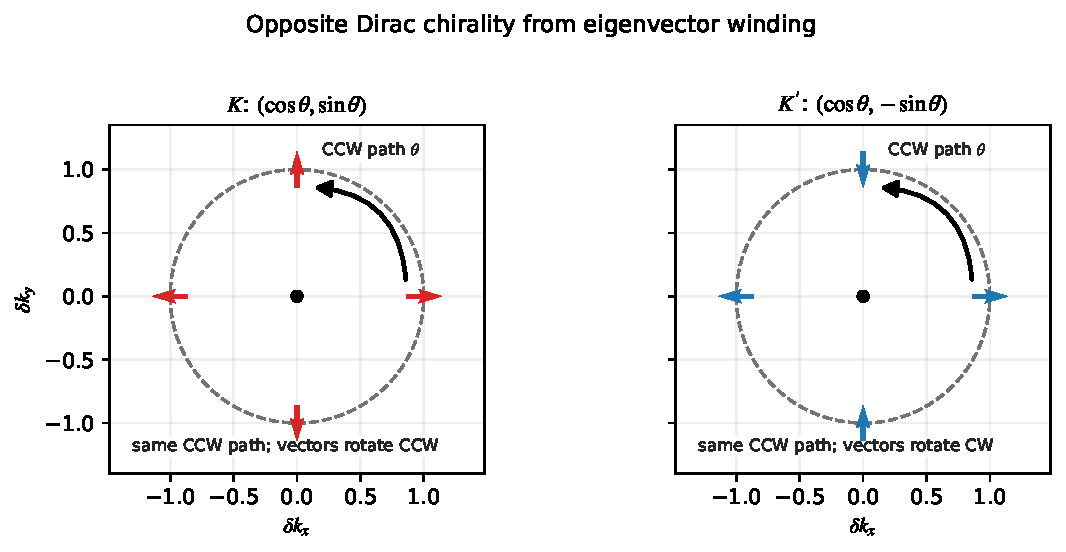
\includegraphics[width=0.92\textwidth]{figures/fig_ch06_dirac_pair_chirality.pdf}
  \caption{Dirac cones occur in opposite-chirality pairs at $K$ and $K'$.
  The two cones have the same local conical spectrum but opposite winding
  orientation in momentum space.  This is the geometric origin of the
  valley-sign bookkeeping used in \secref{sec:ch6-pairs}.}
  \label{fig:ch06-dirac-pair}
\end{figure}

\section{Photonic Dirac semimetals and higher-order crossings}
\label{sec:ch6-dirac-semimetal}

The Dirac cones studied so far in this chapter are two-dimensional:
they occur at isolated $\kvec$-points in the 2D Brillouin zone.
Extending the analysis to three-dimensional photonic crystals reveals
a rich landscape of band crossings protected by crystalline
symmetries.

\subsection{Dirac points in three dimensions}
\label{sec:ch6-3d-dirac}

A Dirac point in a 3D photonic crystal is a fourfold band degeneracy
at which the dispersion is linear in all three momentum directions.
Such degeneracies are protected by the combination of time-reversal
symmetry and a non-symmorphic space group symmetry (e.g.\ a glide
plane or screw axis).  The low-energy effective Hamiltonian near a
3D Dirac point takes the form
\begin{equation}\label{eq:ch6-3d-dirac-hamiltonian}
  H_{\mathrm{Dirac}}^{(3D)}(\delta\kvec) =
  v_1 \delta k_x \alpha_x + v_2 \delta k_y \alpha_y
  + v_3 \delta k_z \alpha_z\,,
\end{equation}
where $\alpha_i$ are $4\times 4$ Dirac matrices and $v_i$ are the
group velocities along the three crystal axes.  Breaking time-reversal
or inversion symmetry splits the Dirac point into two Weyl points
(Chapter~\ref{ch:weyl-points}), each carrying a topological charge
of $\pm 1$ \cite{lu2019experimental,ozawa2018topological}.

\subsection{Quadratic and higher-order band touchings}
\label{sec:ch6-quadratic-touching}

Not all band crossings in photonic crystals are linear.  At
high-symmetry points with enhanced rotation symmetry (e.g.\ the
$\Gamma$ point of a $C_6$-symmetric lattice), bands can touch
quadratically:
\begin{equation}\label{eq:ch6-quadratic-dispersion}
  \omega_\pm(\kvec) = \omega_0 \pm \beta |\kvec|^2 + O(|\kvec|^3)\,,
\end{equation}
where $\beta$ is a curvature parameter determined by the band
structure.  Such quadratic band touchings carry a Berry flux of
$\pm 2\pi$ (instead of $\pm\pi$ for a linear Dirac cone), making
them equivalent to a pair of merged Dirac cones
\cite{wu2015scheme,ozawa2018topological}.

The quadratic band touching is unstable: any perturbation that
lowers the rotation symmetry splits it into two linear Dirac
cones.  This is the mechanism behind the zone-folding construction
of Chapter~\ref{ch:reciprocal-designs}, where a $C_6$-symmetric
photonic crystal is distorted to create a pair of Dirac cones
at the $\Gamma$ point that can then be gapped by further
symmetry breaking \cite{wu2015scheme,kim2020recent}.

The contrast between linear and quadratic touchings is summarised in
Figure~\ref{fig:ch06-linear-quadratic}.  Panels~(a) and~(b) sketch the two
dispersion types along a one-dimensional momentum cut: the linear Dirac cone
$\delta\omega\propto|\delta k|$ and the quadratic touching
$\delta\omega\propto\delta k^2$.  Panels~(c) and~(d) display the corresponding
Berry-curvature magnitude $|\Omega(\kvec)|$ in the two-dimensional Brillouin
zone on a shared logarithmic colour scale.  For the linear case the curvature
is sharply localised at the degeneracy, whereas for the quadratic case it
spreads over a broader region, reflecting the doubled Berry flux $2\pi$ carried
by the merged node.  Both heatmaps assume an isotropic model for visual clarity;
in a real photonic crystal the curvature distribution inherits the lattice
symmetry.

\begin{figure}[t]
  \centering
  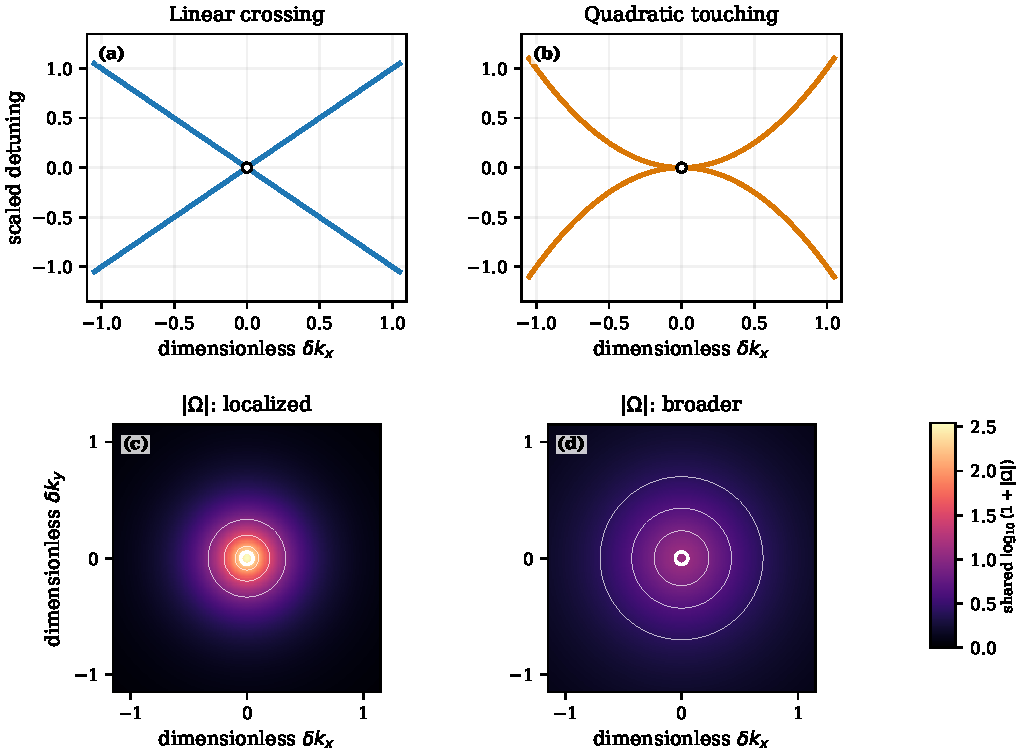
\includegraphics[width=0.95\textwidth]{figures/fig_ch06_linear_quadratic_touching_step178.pdf}
  \caption{Linear versus quadratic photonic band touchings.
  (a)~Linear Dirac cone with Berry flux $\pi$ per cone.
  (b)~Quadratic touching with Berry flux $2\pi$, equivalent to two merged Dirac
  cones.  Open circles mark the degeneracy point.
  (c,\,d)~Normalised Berry-curvature magnitude
  $\log_{10}(1+|\Omega|)$ on a shared colour scale (right-side bar);
  open circles mark the touching point.  The isotropic model is used for
  schematic clarity; realistic photonic crystals exhibit lattice-symmetry
  corrections (Section~\ref{sec:ch6-valley-contrast}).}
  \label{fig:ch06-linear-quadratic}
\end{figure}

\subsection{Valley-contrasting physics and selection rules}
\label{sec:ch6-valley-contrast}

The two inequivalent Dirac cones at $K$ and $K'$ carry opposite
Berry curvature (under inversion-symmetry breaking) and opposite
angular momentum of the Bloch modes.  This valley-contrasting
physics gives rise to selection rules for the coupling between
external radiation and specific valleys: circularly polarised light
couples preferentially to one valley, providing a mechanism for
valley-selective excitation and detection
\cite{dong2016valley,gao2017valley}.

These valley-optical selection rules are the photonic analogue
of the valley-dependent circular dichroism observed in transition
metal dichalcogenides and provide a practical tool for encoding
information in the valley degree of freedom of photonic crystals
\cite{he2016photonic,gao2017topologically}.

\section*{Exercises}

\begin{exercise}
  Show that three free-photon plane waves at a hexagonal BZ corner are
  degenerate by verifying that $|\kvec_K+\Gvec_1|=|\kvec_K+\Gvec_2|
  =|\kvec_K|$.  \emph{Hint:} use the relation
  $\kvec_{K_1}=(\Gvec_2-\Gvec_3)/3$.
\end{exercise}

\begin{exercise}
  Verify that the eigenvalues of the massless Dirac equation
  $v_D(\delta k_x\sigma_x+\delta k_y\sigma_y)|\psi\rangle
  =\delta\omega|\psi\rangle$ are $\delta\omega_\pm=\pm v_D|\delta\kvec|$,
  and compute the eigenstates.
\end{exercise}

\begin{exercise}
  Show that the Berry phase acquired by the eigenstate
  \eqref{eq:ch6-dirac-evec} as $\delta\kvec$ traverses a circle of
  radius $q$ around the Dirac point is $\pm\pi$, independent of $q$.
  Interpret this as the ``monopole charge'' at the degeneracy.
\end{exercise}

\begin{exercise}
  In the electronic context, the von~Neumann--Wigner argument counts
  the number of parameters needed to produce a degeneracy.  Repeat
  this argument explicitly for a general $2\times 2$ matrix that is
  (a) complex Hermitian and (b) real symmetric, and verify that the
  codimensions are 3 and 2, respectively.
\end{exercise}

\begin{exercise}
  Consider a hexagonal photonic crystal with $C_{6v}$ symmetry.  At the
  $K$ point, the little group is $C_{3v}=\{E,C_3,C_3^2,\sigma_v,
  \sigma_v',\sigma_v''\}$.  List the irreducible representations of
  $C_{3v}$, identify which is two-dimensional, and explain why modes
  in this representation are degenerate.
\end{exercise}
